\subsection{Das Grad}

Wie in \cref{sec:int} erwähnt wollen wir uns zunächst mit dem genauen Verhältnis
einer reinen Quinte ($2:3$) beschäftigen. Die Differenz zur gleichstufigen
Quinte,
\[1{.}200\,\on{ct}\cdot \log_2(\tfrac32) - 700\,\on{ct} \approx
  1{,}96\,\on{ct}\]%
wird \emph{Grad} genannt und ist sehr klein (etwa $\frac1{50}$ eines
gleichstufigen Halbtonschrittes), aber dennoch etwas, das wir korrigieren
wollen.

\subsection{Enharmonik}

Ohne die Einschränkungen eines Instruments mit diskreten Tonhöhen kann das Grad
leicht korrigiert werden, sofern wir akzeptieren, dass enharmonisch
unterschiedene Tonhöhen (wie etwa \sharp g und \flat a) verschiedenen Frequenzen
entsprechen können.  Dies mag auf den ersten Blick seltsam erscheinen, aber das
Beispiel aus \cref{fig:enhContext} mag skeptische Leser:innen vielleicht
überzeugen (das Audiobeispiel ist in gleichstufiger Stimmung): In beiden Fällen
ist das resultierende Intervall acht Halbtonschritte groß (\flat e’\,–\,h’ und
\sharp d’\,–\,h’), aber im ersten Fall klingt es dissonant, da der Kontext
nahelegt, dass es aus vier Ganztönen besteht, während es im zweiten Fall
konsonant klingt.

\begin{figure}[h]
  \centering
  \LY{b-enhContext}
  \includegraphics{ly/b-enhContext.pdf}
  \caption{Eine übermäßige Quinte ist keine kleine Sexte.}\label{fig:enhContext}
\end{figure}

\subsection{Die pythagoreische Stimmung}

\noindent Akzeptierend, dass Enharmonik eine Rolle spielt, machen wir uns die
Tatsache zunutze, dass es für jede enharmonisch verschiedene Tonhöhe (c’, \sharp
h und \dflat d’ sind drei unterschiedliche Beispiele!) eindeutig bestimmte ganze
Zahlen $p,q\in\Z$ gibt, für die die gegebene Tonhöhe von a’ aus erreicht werden
kann, indem man $p$ reine Quinten und $q$ Oktaven nach oben geht (eine negative
Zahl bedeutet, dass man nach unten geht). Setzen wir den Kammerton auf $440\Hz$,
so ordnen wir der Tonhöhe die Frequenz $(\frac32)^p\cdot 2^q\cdot 440\Hz$
zu. Ein Beispiel:
\begin{align*}
  \text{\sharp g’}&\equiv(\tfrac32)^5\cdot 2^{-3}\cdot 440\Hz\approx 417.66\Hz,\\
  \text{\flat a’} &\equiv(\tfrac32)^{-7}\cdot 2^4\cdot 440\Hz\approx 412.03\Hz.
\end{align*}

\subsection{Das pythagoreische Komma und die Wolfsquinte}

Der Unterschied zwischen den obigen Frequenzen für \sharp g' und \flat a' heißt
\emph{pythagoreisches Komma} und beträgt
$3^{12}\cdot 2^{-19}\approx 23{,}46\,\on{ct}$. Wir bemerken, dass das
pythagoreische Komma genau $12$ Grad groß ist
($12\cdot 1{,}96\,\om{ct}\approx 23{,}46\om{ct}$), was daran liegt, dass die
beiden enharmonisch verwechselten Töne genau $12$ Quinten (und einige Oktaven)
auseinanderliegen.

Eine verminderte Sexte unterscheidet sich von einer reinen Quinte
notwendigerweise um genau dieses pythagoreische Komma. Eine verminderte Sexte
wird in der pythagoreischen Stimmung manchmal als „Wolfsintervall“ bezeichnet,
da sie sehr verstimmt klingt, siehe \cref{fig:pythComma}:2.

\subsection{Die Quintenspirale}

In \cref{fig:spiral5} ist eine enharmonische Variante des Quintenzirkels zu
sehen, die wir als \emph{Quintenspirale} bezeichnen können. Mit jeder vollen
Runde in dieser Spirale verschiebt sich die Tonhöhe um ein pythagoreisches
Komma, mit jedem Schritt (also $\frac1{12}$ einer Runde) entfernen wir uns um
$1$ zusätzliches Grad von der gleichstufigen Stimmung (oder nähern uns ihr; je
nach dem, in welche Richtung wir gehen).

Da die Töne einer heptatonischen Skala (z.\,B. Dur) einen zusammenhängenden
Abschnitt in dieser Quintenspirale bilden (z.\,B. sind die Töne von C-Dur genau
die von f bis h), sind diese Skalen „in sich“ (also relativ zum Grundton)
beinahe gleichstufig gestimmt: Die größte Abweichung in Dur ist wohl der Leitton
(also der 7. Ton), der pythagoreisch ganze $5$ Grad höher als gleichstufig ist.

\begin{figure}[h]
  \centering
  \includegraphics{ly/b-pythComma}
  \LY{b-pythComma}
  \caption{(1) Der Unterschied zwischen \sharp g’ and \flat a’. (2) Das
    Wolfsintervall \sharp g’\,–\,\flat e’, gefolgt von der reinen Quinte \sharp
    g’\,–\,\sharp d’.}\label{fig:pythComma}
\end{figure}

\subsection{Intervalle in pythagoreischer Stimmung}

Für jedes (enharmonisch präzise angegebenes) Intervall können wir das
entsprechende Frequenzverhältnis berechnen und angeben, um wie viel Grad das
Verhältnis vom gleichstufigen Fall abweicht, siehe \cref{tab:1}.

Wir bemerken, dass diese Tabelle fast alle relevanten Intervalle abdeckt: Wenn
ein bestimmtes Intervall das Verhältnis $a:b$ hat, so hat nämlich sein
\emph{Kom\-plementär\-intervall} das Verhältnis $b:2a$.  Wenn es die Größe $c$ in
Cent hat, so hat sein Komplementärintervall die Größe $1{.}200\,\on{ct}-c$, und
die Abweichung in Grad wechselt das Vorzeichen.  So entspricht eine kleine Sexte
in pythagoreischer Stimmung dem Verhältnis $81:128$, was dasselbe ist wie
$792{,}18\,\on{ct}$ und von der gleichstufigen kleinen Sexte um $-4$ Grad
abweicht.\looseness-1

\begin{figure}
  \centering%
  \newcommand{\pitcharray}{%
  \dflat d, \dflat a, \dflat e, \dflat h, \flat f,
  \flat c, \flat g, \flat d, \flat a, \flat e,
  \flat h, f, c, g, d, a, e, h,
  \sharp f, \sharp c, \sharp g, \sharp d, \sharp a, \sharp e, \sharp h}
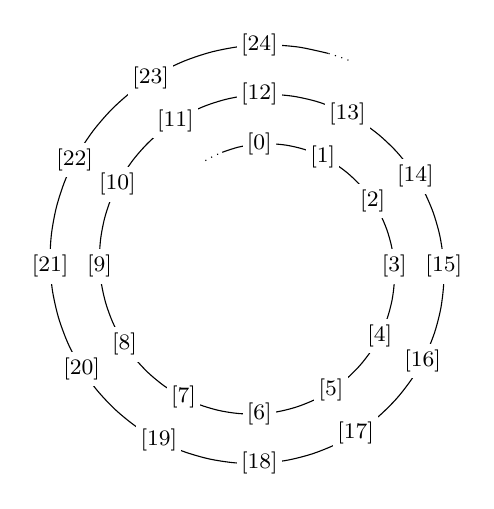
\begin{tikzpicture}[xscale=-1]
  \def\xA{1.4}
  \def\xB{.1}
  \draw[dotted,domain=.35*pi:.4*pi,smooth,samples=100,variable=\t]
  plot ({(\xA+\xB*\t)*cos(\t r)},{(\xA+\xB*\t)*sin(\t r)});
  \draw[domain=.4*pi:4.6*pi,smooth,samples=100,variable=\t]
  plot ({(\xA+\xB*\t)*cos(\t r)},{(\xA+\xB*\t)*sin(\t r)});
  \draw[dotted,domain=4.6*pi:4.63*pi,smooth,samples=100,variable=\t]
  plot ({(\xA+\xB*\t)*cos(\t r)},{(\xA+\xB*\t)*sin(\t r)});
  \foreach \i in {0,...,24}{
    \node[fill=white,inner sep=1.5px]
    at ({(\xA+\xB*(\i+3)*pi/6)*cos((\i+3)*pi/6 r)},
    {(\xA+\xB*(\i+3)*pi/6)*sin((\i+3)*pi/6 r)})
    {\footnotesize \pitch[\i]$\strut$};
  };
\end{tikzpicture}

  \caption{Die enharmonische Quintenspirale. Mit jeder vollen Rotation im
  	Uhrzeigersinn gewinnen wir ein pythagoreisches Komma.}\label{fig:spiral5}
\end{figure}

\begin{table}
  \centering
  \begin{tabular}{lr@{\hspace*{2.4px}}lrr}
    \toprule
    \textsc{intervall} & \multicolumn{2}{c}{\textsc{verhältnis}} & %
    \textsc{größe in ct} & \textsc{abweichung in grad}\\
    \midrule
    kleine Sekunde  & ~~~$243$ & $:256$ &  $90{,}22$ & $-5$\\
    große Sekunde   &      $8$ & $:9$   & $203{,}91$ & $+2$\\
    kleine Terz     &     $27$ & $:32$  & $294{,}13$ & $-3$\\
    große Terz      &     $64$ & $:81$  & $407{,}82$ & $+4$\\
    reine Quarte    &      $3$ & $:4$   & $498{,}04$ & $-1$\\
    \bottomrule
  \end{tabular}
  \caption{Ausgewählte Intervalle in pythagoreischer Stimmung und ihre Differenz
    zur gleichstufigen Stimmung in Grad.}\label{tab:1}
\end{table}

\subsection{Einordnung}

Während alle noch kommenden Mikroalterationen (die darauf abzielen, ganze
Akkorde zu stimmen) den Preis haben werden, dass es mehrere Frequenzen für
denselben Tonnamen gibt, verwendet die bloße pythagoreische Stimmung nur die
Informationen, die uns durch die geschriebenen Noten gegeben werden.
Insbesondere haben in pythagoreischer Stimmung diatonische Halb- und
Ganztonschritte (also kleine und große Sekunde) feste Größen; eine diatonische
Skala in pythagoreischer Stimmung kennt also nur zwei Schrittweiten – eine
Tugend, die durch kontextabhängige Mikroalterationen leider verloren gehen wird.
Daher liegt es bei melodisch gedachten Passagen mit vielen horizontalen
Schritten oft nahe, sie pythagoreisch zu intonieren.

Der entscheidende Nachteil der pythagoreischen Stimmung, der nichts mit der
Realisierbarkeit auf einem diskretisierenden Instrument zu tun hat, sondern rein
theoretischer Natur ist, ist allerdings die Tatsache, dass sie die Unreinheit
der Terzen in einem Dreiklang im Vergleich zur gleichstufigen Stimmung sogar
noch erhöht: Der Unterschied zwischen einer pythagoreischen großen Terz
($407{,}82\,\on{ct}$) und dem oben erwähnten Verhältnis $4:5$
($386{,}31\,\on{ct}$) beträgt $21{,}51\,\on{ct}$. Dieser Fehler ist Gegenstand
des nächsten Abschnitts.

%%% Local Variables:
%%% mode: latex
%%% TeX-master: "../main"
%%% End:
